\setcounter{ExampleCounter}{1}
In essence, linear models start with a simple assumption: growth happens based on adding a fixed amount over and over again.  In this section, we'll investigate exponential models, which are the result of a different assumption, that growth happens by adding a \emph{percentage} of the current total.  In financial terms, this is the difference between simple interest (linear) and compound interest (exponential).

\begin{center}

\includegraphics[width=0.8\textwidth]{geese}
\end{center}

Many of the examples in this section deal with population growth, because this is a decent assumption to start with.  Since the number of offspring in one generation depends on the number of parents in the previous generation, it makes sense that as the population grows, the number of offspring grows as well.\\

For instance, suppose that in order to predict the population of geese in a particular area, you assume that the number of geese will increase by 10\% each year (accounting for births and deaths).  According to this model, an initial population of 1000 geese would grow to 1100 geese at the end of one year, and the following year, 10\% of 1100 would be added, making the growth speed up.

Notice that adding 10\% to the total is the same as multiplying by 110\%, or 1.1:
\[1000 + 1000(0.1) = 1000(1+0.1) = 1000(1.1)\]

We can track this for a few years, multiplying each year's population by 1.1 to get the next year's result, and watch a formula emerge.
\begin{center}
\begin{tabular}{l l}
Year 0: \hspace*{0.25in} & $P_0 = 1000$\\
Year 1: & $P_1 = 1000(1.1)$\\
Year 2: & $P_2 = 1000(1.1)(1.1)$\\
Year 3: & $P_3 = 1000(1.1)(1.1)(1.1)$
\end{tabular}
\end{center}

It doesn't take long to recognize that each year's population will be 1000 multiplied by 1.1 over and over again.  The number of times that 1.1 is multiplied is the same as the number of years that have elapsed since we started tracking the population.

We can write this more compactly by taking advantage of exponential notation, since for instance, $1000(1.1)(1.1)(1.1) = 1000(1.1)^3$.

In our example, then, we could predict the population of geese in any year using the following formula:
\[P_t = 1000(1.1)^t\]

The \textbf{growth rate} is 10\%, and 1.10 is the \textbf{growth multiplier}.  Each year's population is 1.10 times the previous year's population.

\begin{center}
\begin{tabular}{c | c | c}
\textbf{Year} & \textbf{Population} & \textbf{Growth from Previous Year}\\
\hline
0 & 1000 &\\
1 & 1100 & 100\\
2 & 1210 & 110\\
3 & 1331 & 121\\
4 & 1464 & 133\\
5 & 1611 & 147\\
6 & 1772 & 161
\end{tabular}
\end{center}
Notice that there is a constant \textit{percentage} growth, so as the population increases, the number by which it grows gets larger each year.\\

If we plot these first few values, the graph is not quite linear, but it's not that far from a linear plot.  Because of this, in the short term, linear models can approximate exponential models, even if it isn't a perfect fit.
\begin{center}
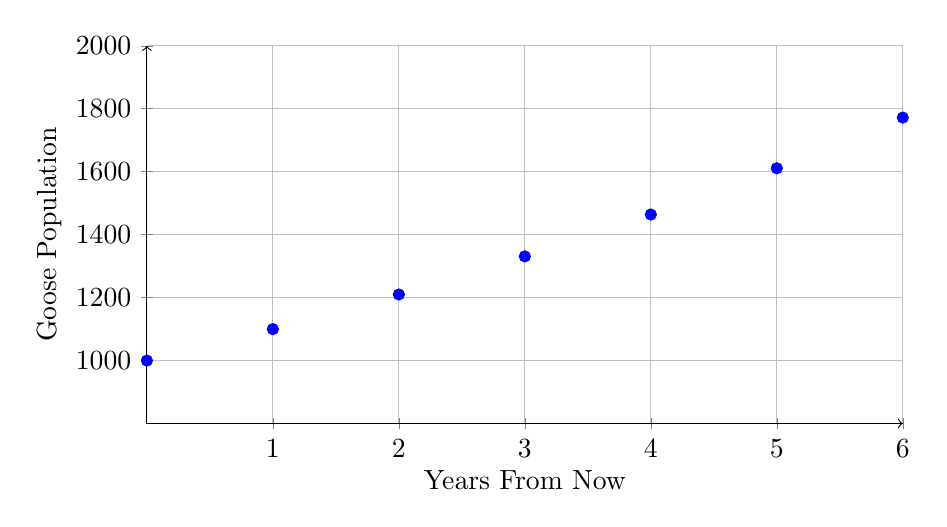
\begin{tikzpicture}
\begin{axis}[
    xmin=0, xmax=6,
    ymin=800, ymax=2000,
    axis lines=center,
    axis on top=false,
    domain=0:1,
    x=1.6cm,
    y=0.004cm,
    xtick={0,1,...,6},
    xticklabels={0,1,...,6},
    ytick={0,200,...,2000},
    yticklabels={0,200,...,2000},
    axis lines=middle,
    axis line style={->},
    x label style={at={(axis description cs:0.5,-0.1)},anchor=north},
    y label style={at={(axis description cs:-0.1,.5)},rotate=90,anchor=south},
    xlabel={Years From Now},
    ylabel={Goose Population},
    grid=major
    ]
	\addplot [blue,only marks] table {
	0 1000
	1 1100
	2 1210
	3 1331
	4 1464
	5 1611
	6 1772
	};
\end{axis}
\end{tikzpicture}
\end{center}

As we begin to project further into the future, though, the model clearly deviates from a linear trend:
\begin{center}
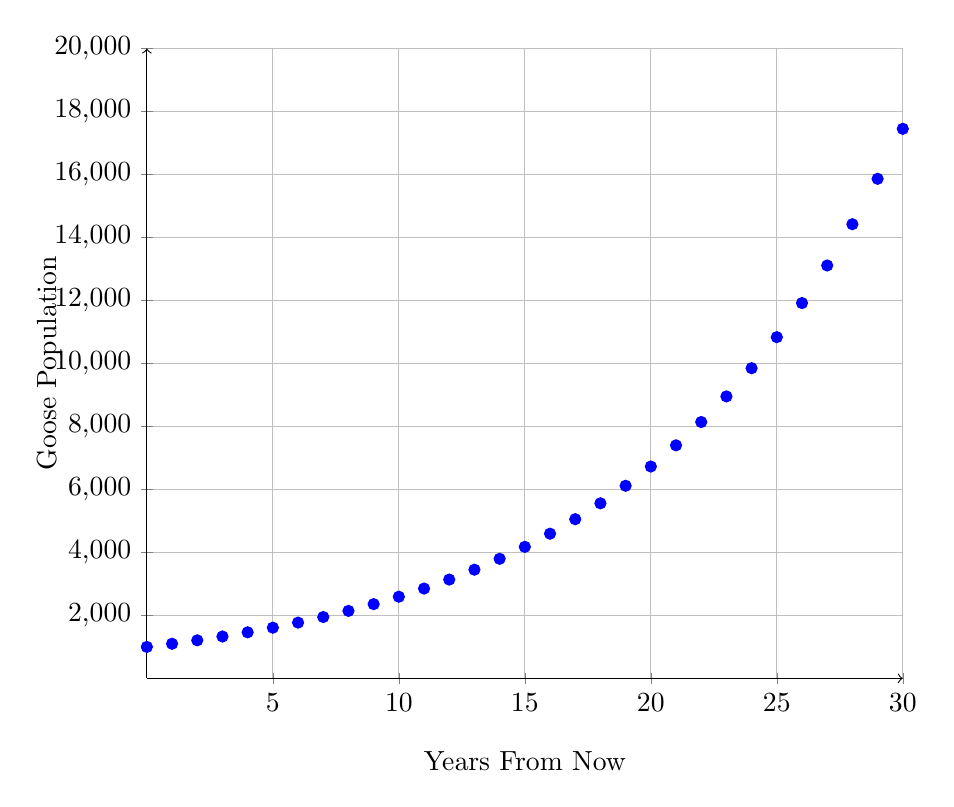
\begin{tikzpicture}
\begin{axis}[
    xmin=0, xmax=30,
    ymin=0, ymax=20,
    axis lines=center,
    axis on top=false,
    domain=0:1,
    x=0.32cm,
    y=0.4cm,
    xtick={0,5,...,30},
    xticklabels={0,5,...,30},
    ytick={0,2,...,20},
    yticklabels={0,{2,000},{4,000},{6,000},{8,000},{10,000},{12,000},{14,000},{16,000},{18,000},{20,000}},
    axis lines=middle,
    axis line style={->},
    x label style={at={(axis description cs:0.5,-0.1)},anchor=north},
    y label style={at={(axis description cs:-0.1,.5)},rotate=90,anchor=south},
    xlabel={Years From Now},
    ylabel={Goose Population},
    grid=major
    ]
	\addplot [blue,only marks] table {
	0 1
	1 1.1
	2 1.21
	3 1.331
	4 1.464
	5 1.611
	6 1.772
	7 1.949
	8 2.144
	9 2.358
	10 2.594
	11 2.853
	12 3.138
	13 3.452
	14 3.798
	15 4.177
	16 4.595
	17 5.055
	18 5.56
	19 6.116
	20 6.728
	21 7.4
	22 8.14
	23 8.954
	24 9.85
	25 10.835
	26 11.918
	27 13.11
	28 14.421
	29 15.863
	30 17.45
	};
\end{axis}
\end{tikzpicture}
\end{center}

If the population had been growing linearly by 100 geese each year, the population at the end of 30 years would have only been 4,000 instead of nearly 18,000 under the exponential model.  Most of this growth occurred in the second half; this is typical of exponential growth.  Since the growth from one year to another depends on the size of the population, it grows much faster near the end, and the growth begins to snowball.

\begin{formula}{Exponential Growth}
If a quantity starts at size $P_0$ and grows by $R\%$ (written as a decimal, $r$) every time period, then the quantity after $t$ time periods is given by
\[P_t = P_0 (1+r)^t\]
The \textbf{growth rate} is $r$, and the \textbf{growth multiplier} is $1+r$.\\

If $r$ is negative, then instead of exponential growth there is \textbf{exponential decay}.
\end{formula}

The growth multiplier is the common ratio between terms, and it can be used to recognize exponential growth from data, just like a common difference between terms can be used to recognize linear growth.
\begin{center}
\begin{tabular}{c c c}
\textbf{Year} & \textbf{Population} & \textbf{Ratio to Previous Year}\\
\hline
& & \\
0 & 1000 &\\
1 & 1100 & 1.1\\
2 & 1210 & 1.1\\
3 & 1331 & 1.1\\
4 & 1464 & 1.1\\
5 & 1611 & 1.1\\
6 & 1772 & 1.1
\end{tabular}
\end{center}

\paragraph{Picking the Model Type}
How do we know whether to use a linear, quadratic, or exponential model (or some other type)?  This is not a simple question, so in this chapter you will always be told what type of model to use.

However, we can look briefly at a simple example to see how this question may be answered.  There are statistical tools that can be used to pick a model, but for now, we'll restrict ourselves to simply inspecting the data and doing a quick visual check.

First, to distinguish between linear and exponential models, calculate the difference between each year's population and the next, and the ratio of the two populations.  If the difference is roughly consistent, try a linear model.  If, instead, the ratio is relatively unchanged, try an exponential model.  Quadratic models are not as easy to observe this way, but in general, quadratic models fall somewhere between the other two.

Then, draw a scatterplot of the data and see if you can observe a trend.  The more data you have available, the easier this is.  Of course, this is not foolproof.  For instance, consider the data graphed below.
\begin{center}
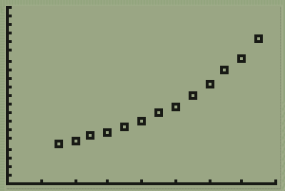
\includegraphics[width=2in]{PickingModelType1}
\end{center}

This data doesn't necessarily look linear, but we could certainly find a linear model to approximate it, and it wouldn't be completely ridiculous.

We can compare the three types of models, and plot the results against the data:
\begin{center}
\begin{tabular}{c c c}
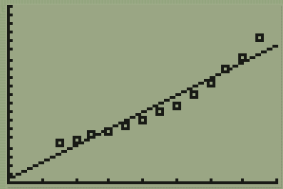
\includegraphics[width=1.3in]{PickingModelType2}
& 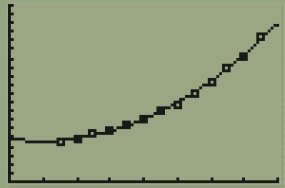
\includegraphics[width=1.3in]{PickingModelType3}
& 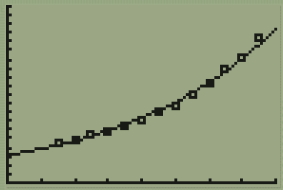
\includegraphics[width=1.3in]{PickingModelType4}\\
Linear & Quadratic & Exponential
\end{tabular}
\end{center}

It looks like the quadratic and exponential models track the data better than the linear one, but between the two leaders, which is better?  There's no clear answer, so we could probably pick either one and get decent results.  In fact, trying out a bunch of models in the hopes of finding a perfect one can lead to \emph{overfitting}, which happens when our entire focus is on explaining the data from the past, rather than being able to predict future results.
\pagebreak

\begin{example}[https://www.youtube.com/watch?v=NHLi7ekPSPM]{Frederick Population}
The population of Frederick County grew from 239,520 in 2012 to 241,409 in 2013, a growth of about 0.8\%.  If this growth rate continues, what is the population of Frederick County expected to be in 2025?

\solline
\marginnote{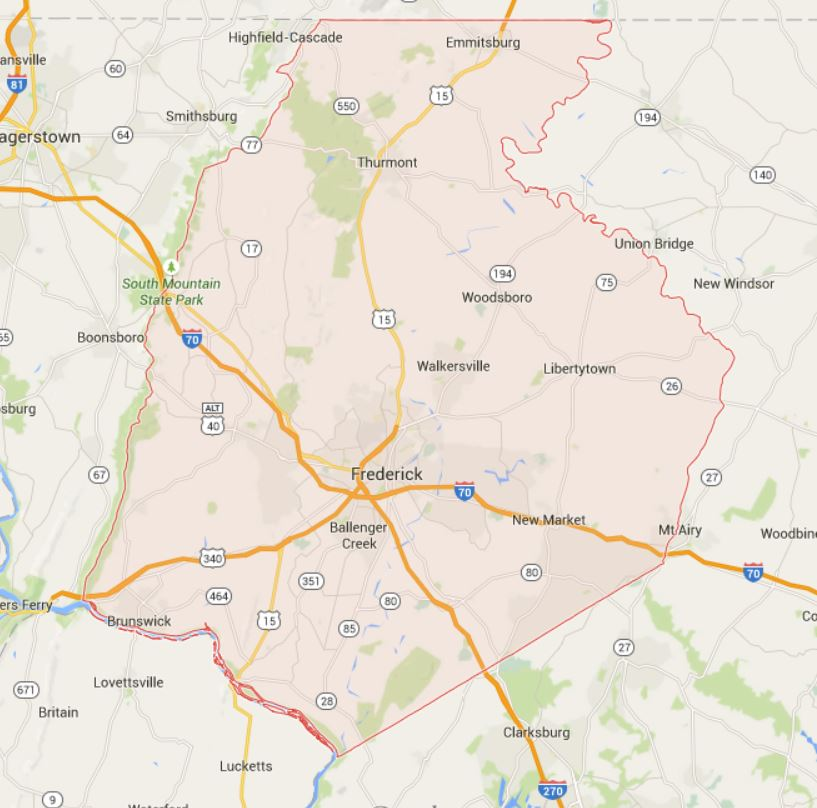
\includegraphics[scale=0.15]{FrederickCountyMap1}}
If $r=0.008$, we can use the exponential growth formula to predict the population in 2025.  To do so, however, we need to pick a year to be year 0.  Since we're given the population in 2012 and 2013, we can use either one, but we'll choose 2013, so 2025 will be year 12.
\begin{align*}
P_{12} &= P_0 (1+r)^t\\
&= 241,409(1+0.008)^{12}\\
&= \boxed{265,632}
\end{align*}
We expect the population of Frederick County to reach 265,632 by 2025.
\end{example}

\begin{try}[http://www.izzomath.com/103text/growthmodels/example2.1/story.html]
\begin{tabular}{c c}
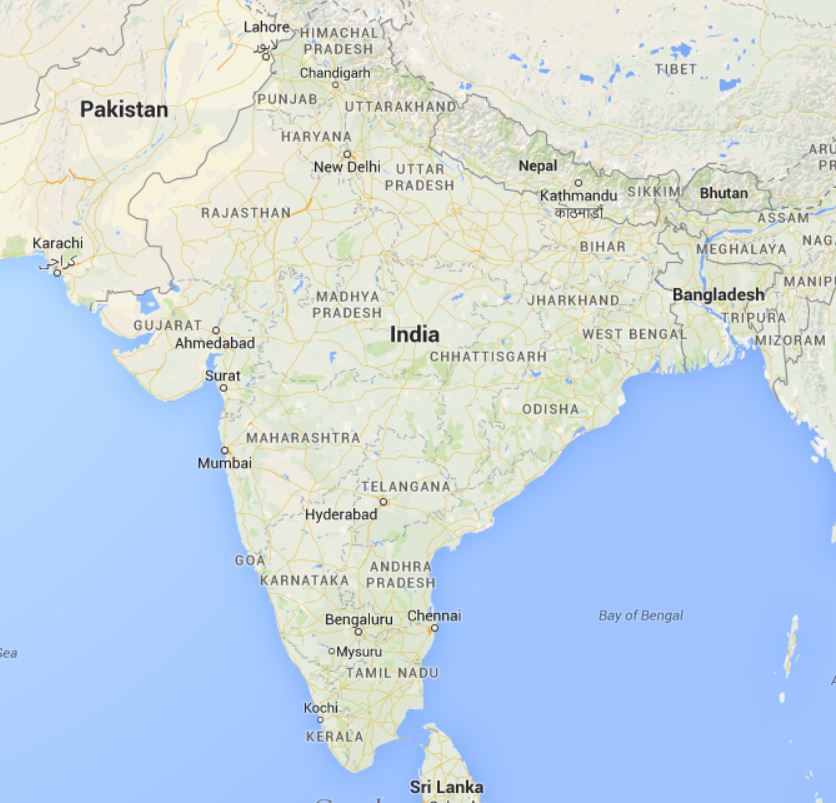
\includegraphics[width=0.3\textwidth]{IndiaMap1} & 
\parbox[b]{2.5in}{India is the second most populous country in the world, with a population of about 1.252 billion in 2013.  The population is growing by about 1.21\% each year.\\

If this trend continues, what is India's population expected to grow to by 2030?}
\end{tabular}
\end{try}

\begin{proc}{Using Your Calculator: Exponents}
\begin{tabular}{c l}
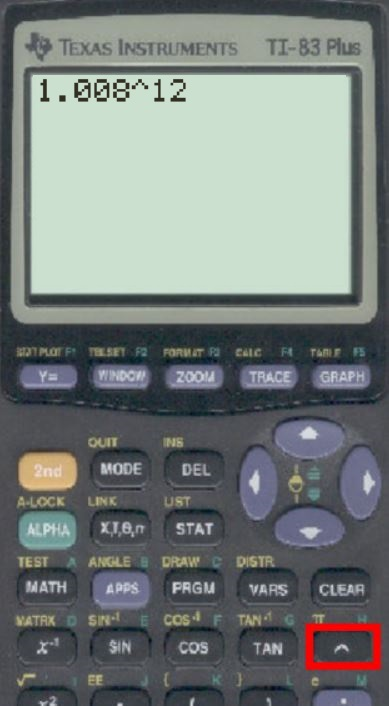
\includegraphics[scale=0.35]{Calculator2} & \parbox[b]{3in}{To evaluate expressions like $1.008^{12}$, we'll use the exponent function on a calculator rather than multiplying 1.008 by itself 12 times.  The exponent function is usually labeled like one of the following:
\begin{center}
\begin{tabular}{c c c}
$\boxed{\wedge}$ & $\boxed{y^x}$ & $\boxed{x^y}$
\end{tabular}
\end{center}

To evaluate $1.008^{12}$, we'd type $1.008 \ \boxed{\wedge}\ 12$ or $1.008\ \boxed{y^x}\ 12$.  Try it and make sure that you get an answer around 1.100338694.}
\end{tabular}
\end{proc}
\pagebreak

\begin{example}[https://www.youtube.com/watch?v=_u9RlZX_BkI]{Tuition Prediction}
A friend is using the equation \[P_t = 4600(1.072)^t\] to predict the annual tuition at a local college.  She says that the formula is based on years after 2010.  What does this equation tell us?

\sol
In this equation, $P_0 = 4600$, which is the initial tuition, so we infer that the tuition in 2010 is \$4600.\\

The growth multiplier is 1.072, so the growth rate is 0.072 or 7.2\%.  We expect tuition to grow by 7.2\% each year.
\end{example}

In reality, we don't generally start a study already knowing the growth rate, as we did in the last few examples.  Instead, we'll start with historical data, and we need to know how to use that to discover the growth rate.

We'll do this in a similar way to what we did in the section on Linear Models.  If you remember, in that section, we had two ways to find the linear growth rate:
\begin{itemize}
\item Use two points from the data set (by default, the first and last points) to calculate the growth rate manually; this requires some algebra.
\item Use all the points in the data set; use the calculator for this, since the details are complex.
\end{itemize}

With quadratic models, we defaulted to the second option and avoided the manual option altogether.  However, we will see one example of finding $r$ manually here, simply to see that it is doable.  The algebra is a bit more complicated than it was for linear models, but still within grasp.

\subsection{Finding the Growth Rate Manually}

For a simple example, suppose that we knew that the population grew from 100 to 200 in 5 years.  We can call 100 the initial population:
\[P_t = 100(1+r)^t\]
The key is that we know a value of $t$ and the corresponding population, $P_t$.  If we substitute these into the equation, there will only be one unknown, $r$, and we can solve for it:
\[200 = 100(1+r)^5\]

The steps to solve for $r$ may be hard to follow at first, but you can use the exact same steps any time you need to solve one of these problems manually.\\

Remember that to solve an equation, we need to strip away everything except the piece we want.  Here, we want to extract $r$, so we need to remove everything around it by undoing whatever operations apply.  This also gives us an idea of the order, since we need to undo operations in the opposite order that we would simplify them according to PEMDAS (parentheses, exponents, multiplication, division, addition, subtraction).

Notice what's happening to $r$: it is added to 1 inside parentheses; since parentheses come first in the order of operations, we'll deal with this last as we solve for $r$.  Next, this is raised to the fifth power, so we'll need to undo this second-to-last.  Finally, the result is multiplied by 100, so we'll start by undoing that.  Here's our process:
\begin{enumerate}
\item Undo multiplication by 100: divide both sides by 100
\item Undo raising to the 5th power: take the 5th root of both sides
\item Undo addition to 1: subtract 1 from both sides
\end{enumerate}

That second step is the one that may be new to you, and it's likely the step that will give you the most trouble.
\pagebreak

Let's see this in action.

\begin{example}[https://www.youtube.com/watch?v=2wtJ_T3_e7o]{Carbon Dioxide Emissions}
In 1990, the residential energy use in the US was responsible for 962 million metric tons of carbon dioxide emissions.  By the year 2000, that number had risen to 1182 million metric tons.  If the emissions grow exponentially and continue at the same rate, what will the emissions grow to by 2050?

\solline
\marginnote{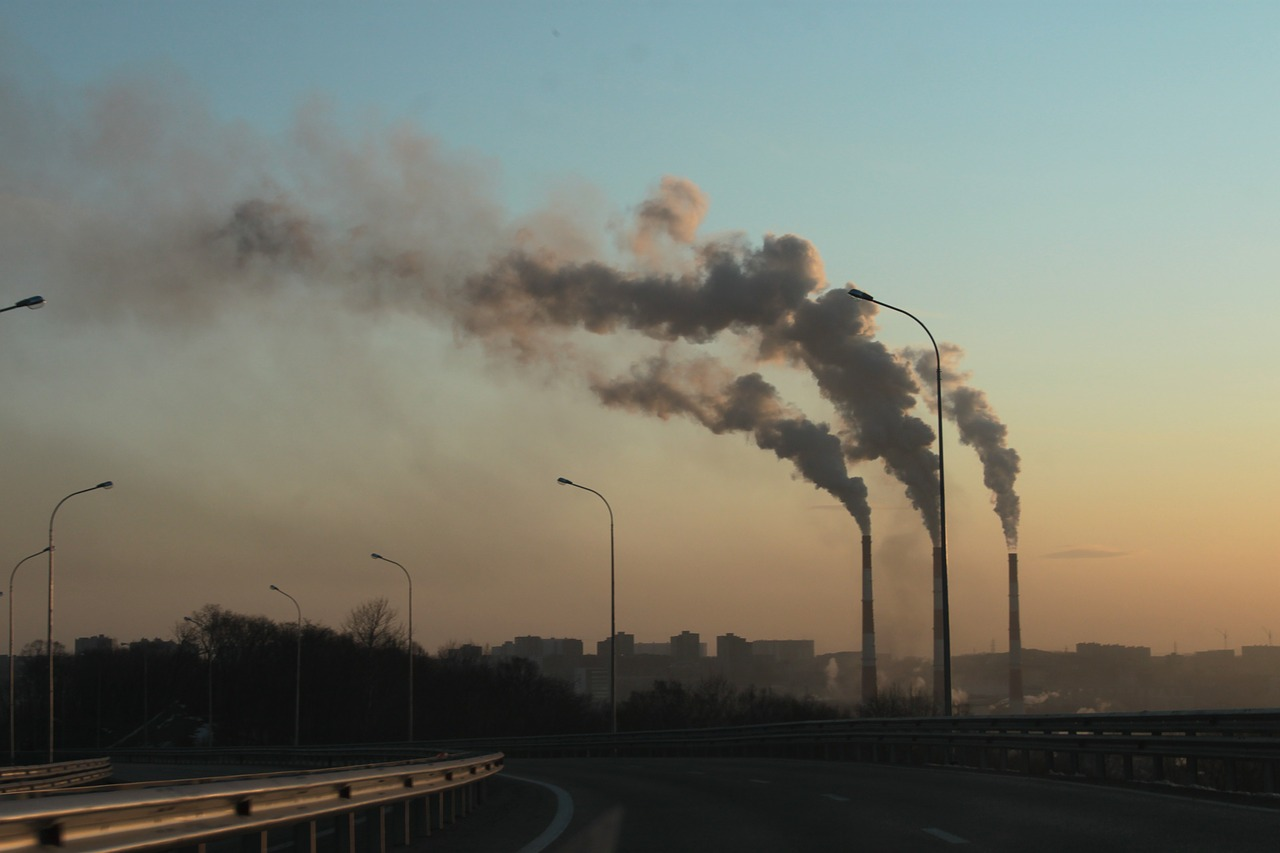
\includegraphics[scale=0.08]{Factory1}}
The twist in this problem is that the growth rate is not explicitly given, so we'll have to find it before we can make our prediction.\\

We will let 1990 correspond to year 0, so 2000 is year 10.
\begin{center}
\begin{tabular}{c c}
\textbf{Year} & \textbf{Emissions (million tons)}\\
\hline
& \\
0 & 962\\
10 & 1182
\end{tabular}
\end{center}
We can put this information into the exponential growth model:
\begin{align*}
P_{10} &= P_0(1+r)^{10}\\
1182 &= 962(1+r)^{10}
\end{align*}

Now we need to solve for $r$:
\begin{center}
\begin{tabular}{c l}
$1182 = 962(1+r)^{10}$ & \\
& \\
$\dfrac{1182}{962} = (1+r)^{10}$ & Divide both sides by 962\\
& \\
$\sqrt[10]{\dfrac{1182}{962}} = 1+r$ & Take the 10th root of both sides\\
& \\
$\sqrt[10]{\dfrac{1182}{962}}-1 = r$ & Subtract 1 from both sides
\end{tabular}
\end{center}
\[r=\sqrt[10]{\dfrac{1182}{962}}-1 = 0.0208 = 2.08\%\]

So if the emissions are growing exponentially, they are growing by about 2.08\% per year.  We can use this to predict the emissions in 2050, using 1990 as year 0:
\[P_{60} = 962(1+0.0208)^{60} = \boxed{2208.4 \textrm{ million metric tons of CO}_2 \textrm{ in 2050}}\]
\end{example}

\begin{try}
The number of users on a social networking site was 45,000 in February when they officially went public, and grew to 60,000 by October.  If the site is growing exponentially and growth continues at the same rate, how many users should they expect two years after they went public?
\end{try}

\paragraph{Rounding:} If we had rounded the growth rate to 2.1\%, our calculation for the emissions in 2050 would have been 3347.  Rounding to 2\% would have given a result of 3156.  A very small difference in the growth rate gets magnified greatly in exponential growth.  Thus, round the growth rate as little as possible, keeping at least three significant digits (numbers after any leading zeros).  For instance, 0.41624 could be reasonably rounded to 0.416, and a growth rate of 0.001027 could be rounded to 0.00103.

\paragraph{Another note:} Here we used two points to build an exponential model.  If all we have is two data points, there's no reason necessarily to use an exponential model; a linear or quadratic model can fit two points just as well.  This only makes sense when we have prior knowledge that convinces us that the growth in this instance will be exponential (like with population or things that are closely linked to it, such as pollution).

\begin{proc}{Using Your Calculator: Roots}
In the previous example, we had to calculate the 10th root of a number.  Many scientific calculators have a button for general roots that looks like:
\begin{center}
\begin{tabular}{c c c}
$\boxed{\sqrt[n]{\hspace{0.1in}}}$ & $\boxed{\sqrt[x]{\hspace{0.1in}}}$ & $\boxed{\sqrt[y]{x}}$
\end{tabular}
\end{center}

To evaluate the 3rd root of 8, for example, we'd type either 3 $\boxed{\sqrt[n]{\hspace{0.1in}}}$ 8 or 8 $\boxed{\sqrt[n]{\hspace{0.1in}}}$ 3, depending on the calculator.  Try it on yours to see---you should get 2.\\

If you can't find a general root button, you can use the property of exponents that \[\sqrt[n]{a} = a^{1/n}.\]
To compute $\sqrt[3]{8}$, then, you could use the exponent key on your calculator to evaluate $8^{1/3}$.  Make sure that you use parentheses to preserve order of operations:
\[8\ \boxed{y^x}\ (\ 1\ \boxed{\div}\ 3\ )\]
\end{proc}

\subsection{Finding the Growth Rate Using a Calculator}
We can use the calculator for an example like the last one, without even resorting to regression (which we'll do a bit later).  Remember that we used the intersect tool to solve for $t$ in earlier models; we can do the same here to solve for $r$.\\

All we need is to graph both sides of the equation, using $x$ instead of $r$:
\begin{center}
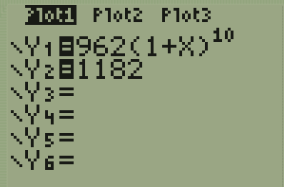
\includegraphics[width=2in]{CalculatorFindR1}
\end{center}

Then use the intersect feature (press \calcbutton{2ND} \calcbutton{TRACE} to access the menu).  Note that in order to visualize the intersection, we set the window for $x$ values to be from 0 to 0.05 (since the growth rate is somewhere below 5\% in this example) and $y$ values between 900 and 1200.  It may take some trial and error to get the window right, but this is not a crucial step of the process; the calculator can find an intersection even if it isn't visible.
\begin{center}
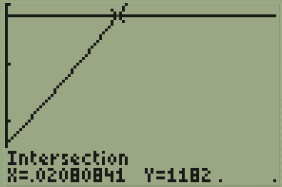
\includegraphics[width=2in]{CalculatorFindR2}
\end{center}

Notice that the value the calculator gives for $x$ is what we were looking for, since we used $x$ to represent $r$: the growth rate is $2.08\%$, just as we found manually.\\

Now that you know how to do this, try going back to the first example, with the population of Frederick County, and try to calculate the growth rate that's given using either manual method or the calculator (or both, for practice).
\pagebreak

\subsection{Solving for Time}
There's nothing new to say about solving for time using the calculator; we've already done this with the previous models in earlier sections, and we just used the same procedure to solve for the growth rate.  However, we'll include an example here, just to remind you how this works.

\begin{example}{Solving for Time}
In the first example, we modeled the population growth of Frederick County from 2013 onward using the following equation:
\[P_t = 241,409(1+0.008)^t\]
Using this model, predict when the population will reach 400,000 people.

\sol
First, let's draw a graph to estimate the answer (an estimate like this may be all we need in some cases).
\begin{center}
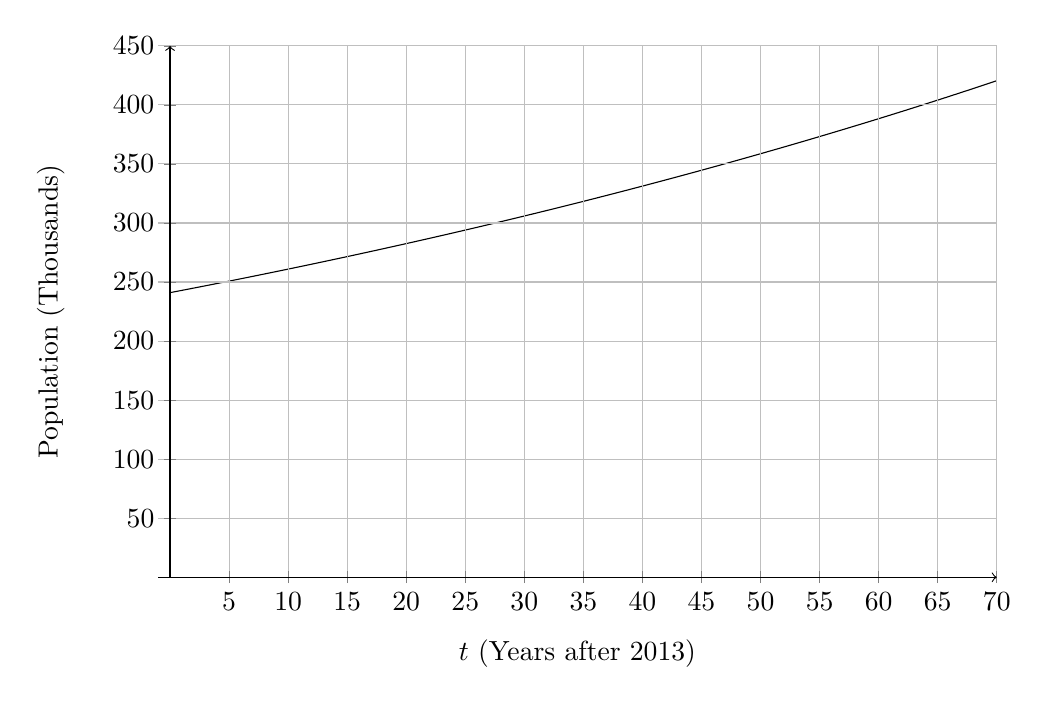
\begin{tikzpicture}
\begin{axis}[
    xmin=-1, xmax=70,
    ymin=0, ymax=450,
    axis lines=center,
    axis on top=true,
    domain=0:1,
    x=0.15cm,
    y=0.015cm,
    xtick={0,5,...,100},
    xticklabels={0,5,...,100},
    ytick={0,50,...,450},
    yticklabels={0,50,...,450},
    axis lines=middle,
    axis line style={->},
    x label style={at={(axis description cs:0.5,-0.1)},anchor=north},
    y label style={at={(axis description cs:-0.1,.5)},rotate=90,anchor=south},
    xlabel={$t$ (Years after 2013)},
    ylabel={Population (Thousands)},
    grid=major
    ]
	\addplot[samples=100,domain=0:70] {241*(1.008^x)};
\end{axis}
\end{tikzpicture}
\end{center}

We can tell that the answer will be somewhere between 60 and 65 years after 2013.  If we pick 63 as a reasonable guess, that means we expect the population to reach 400,000 around the year 2076.\\

To get a more precise guess (but remember, this is still an estimate, so there's no guarantee it will be more accurate than our first one), we can plot the model as well as the horizontal line at 400,000 and find their intersection:
\begin{center}
\begin{tabular}{c c c}
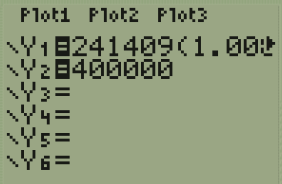
\includegraphics[height=0.9in]{FrederickFindT1}
& 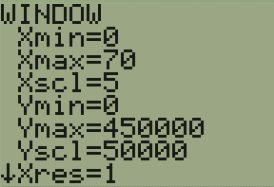
\includegraphics[height=0.9in]{FrederickFindT2}
& 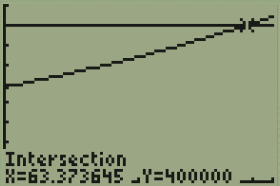
\includegraphics[height=0.9in]{FrederickFindT3}
\end{tabular}
\end{center}

Notice that the intersection occurs around $x=63.4$, so our initial guess of 63 was pretty close.  Thus, we'll stick with 2076 as the year that we predict the population will reach 400,000.
\end{example}

\begin{try}
Using the carbon emissions model from Example 3, predict when the emissions will reach 1500 million metric tons of carbon dioxide.
\end{try}
\pagebreak

\subsection{Exponential Regression}
If we want to use more than two points to find an exponential model, we need to turn to the calculator.  Thankfully, since we've already done linear and quadratic regression, there's not much to add here.  Exponential regression can be found in the same menu, labeled \texttt{0: ExpReg}.  Press the \calcbutton{STAT} button, then scroll to the right to the \texttt{CALC} menu:
\begin{center}
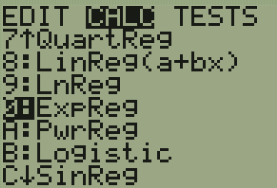
\includegraphics[width=2in]{ExpRegMenu}
\end{center}

The rest of the steps are familiar; start by entering data (with time in the first column and population in the second column), then access the \texttt{ExpReg} function, and leave the default options alone.

\begin{example}{Exponential Regression}
Build an exponential population model for the U.S. using data from 2005 to 2019.

\sol
We need to gather some data first; a quick Internet search yields the following population values:
\begin{center}
\begin{tabular}{c c}
\textbf{Year} & \textbf{Population (in millions)}\\
\hline
& \\
2005 & 295.5\\
2006 & 298.4\\
2007 & 301.2\\
2008 & 304.1\\
2009 & 306.8\\
2010 & 309.3\\
2011 & 311.6\\
2012 & 313.9\\
2013 & 316.1\\
2014 & 318.4\\
2015 & 320.7\\
2016 & 323.1\\
2017 & 325.1\\
2018 & 327.2\\
2019 & 328.2
\end{tabular}
\end{center}

Enter this into the calculator, using 2005 as year 0 (so 2019 will correspond to year 14), and use the exponential regression solver.
\begin{center}
\begin{tabular}{c c c}
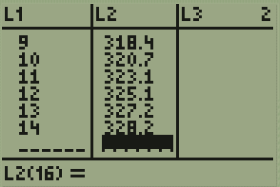
\includegraphics[height=0.8in]{ExpRegEx1}
& 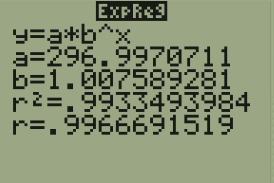
\includegraphics[height=0.8in]{ExpRegEx2}
& 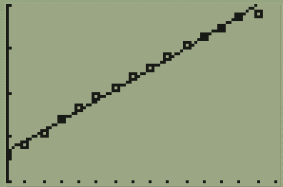
\includegraphics[height=0.8in]{ExpRegEx3}
\end{tabular}
\end{center}

The exponential model is \[\boxed{P_t = 297(1.0076)^t}\] which means that the growth rate is 0.76\%.  We could then use this model to make predictions, as we've done in the last few examples.
\end{example}

\begin{try}
Pick another country, and build an exponential population model using data from the same years.
\end{try}
\pagebreak

\subsection{Using Excel}
We've used Excel to build regression equations for linear and quadratic models; using the same process, you'll notice an option for an exponential model.  We could do it that way; however, the form that Excel gives for the exponential model uses the natural base $e$, which we haven't addressed in this section.  To avoid confusion, we'll use a different process to get a more familiar form; there's a built-in formula called \texttt{LOGEST}, which takes a range of $y$-values and a range of $x$-values, in that order, and returns an exponential model in the form $y=a(b)^x$, just like the graphing calculator.

First, record the data and insert a scatterplot, as before.
\begin{center}
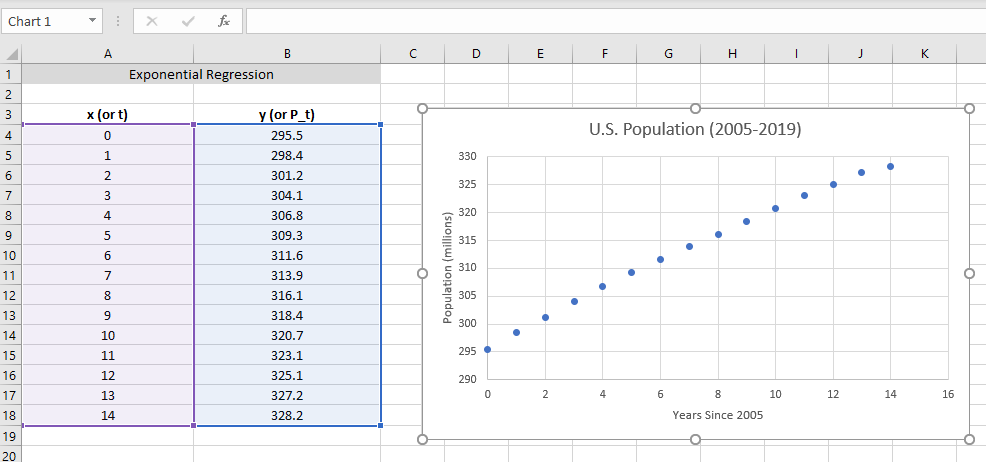
\includegraphics[width=0.8\textwidth]{ExpRegExcel1}
\end{center}

Next, select a cell (\texttt{A24} on the example spreadsheet) and enter the formula
\begin{center}
\texttt{=LOGEST(B4:B18,A4:A18)}
\end{center}
This selects the values in the second column as $y$ and the first column as $x$; the output is shown below.
\begin{center}
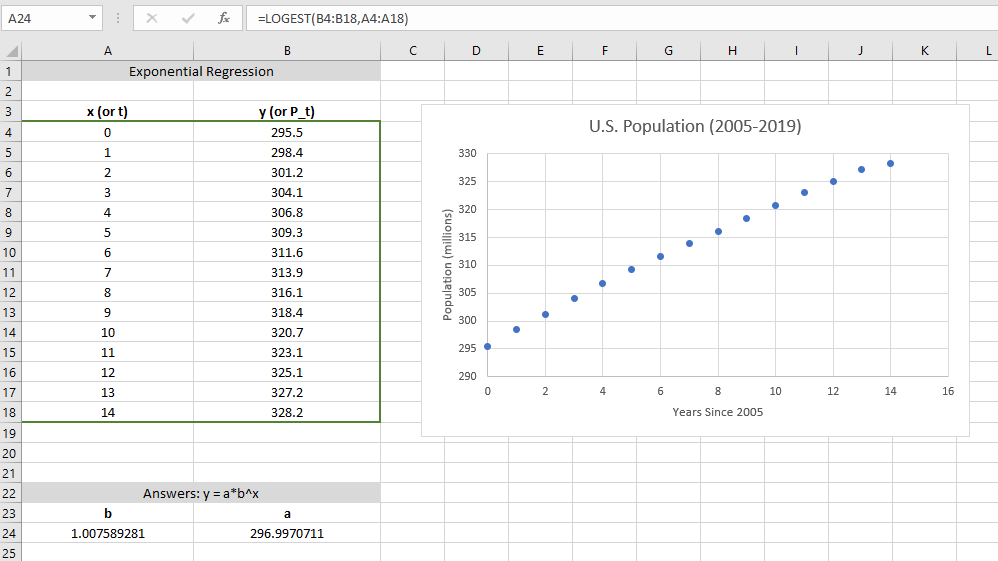
\includegraphics[width=0.8\textwidth]{ExpRegExcel2}
\end{center}

Notice that the output of the formula places the answer for the base of the exponent in the selected cell, and the answer for the initial population in the next cell to the right.

The model given here is 
\[P_t = 297(1.0076)^t\] which is identical to the one from the graphing calculator.